\section{Polynomial Functions}
\label{sec:polynomial}

\subsection{Quadratic Functions}
\label{ssec:quadratic}
% From Section 1.5.

Quadratics are transformations of the function $f(x)=x^2$. Quadratics commonly arise from problems involving area and projectile motion, providing some interesting applications.

\begin{example}
A backyard farmer wants to enclose a rectangular space for a new garden. She has purchased 80 feet of wire fencing to enclose three sides, and will put the fourth side against the backyard fence. Find a formula for the area enclosed by the fence if the sides of fencing perpendicular to the existing fence have length $L$.

\begin{solution} In a scenario like this involving geometry, it is often helpful to draw a picture. It might also be helpful to introduce a temporary variable, W, to represent the side of fencing parallel to the fourth side or backyard fence.
	\begin{figure}[!ht]
	\centering
	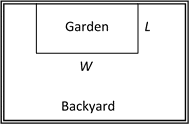
\includegraphics[width=0.4\textwidth]{img/chap1/sec1-5/image096.png}
	\caption{}
	\end{figure}
Since we know we only have 80 feet of fence available, we know that $L+W+L=80$, or more simply, $2L+W=80$. This allows us to represent the width, $W$, in terms of $L$: $W=80-2L$.

Now we are ready to write an equation for the area the fence encloses. We know the area of a rectangle is length multiplied by width, so $A=LW=L(80-2L)$, so
$$A(L)=80L-2L^2 \enspace .$$
This formula represents the area of the fence in terms of the variable length $L$.
\end{solution}\end{example}

\begin{definition}[Forms of Quadratic Functions]
The {\bf standard form} of a {\bf quadratic function}\index{Function!quadratic} is $f(x)=ax^2+bx+c$.

The {\bf transformation form} of a quadratic function is $f(x)=a(x-h)^2+k$.

The {\bf vertex}\index{Vertex} of the quadratic function is located at the point $(h,k)$, where $h$ and $k$ are the numbers in the transformation form of the function. Because the vertex appears in the transformation form, it is often called the {\bf vertex form}.
\end{definition}
\begin{example}
Write an equation for the quadratic graphed below as a transformation of $f(x)=x^2$.

\begin{figure}[!ht]
\centering
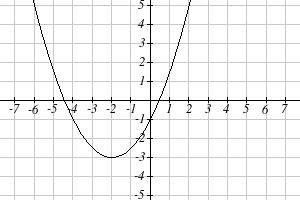
\includegraphics[width=0.4\textwidth]{img/chap1/sec1-5/image057.png}
\caption{}
\end{figure}
\begin{solution} We can see the graph is the basic quadratic shifted to the left 2 and down 3, putting the vertex at the point $(-2,-3)$, giving a formula in the form $g(x)=a(x+2)^2-3$. By plugging in a point that falls on the grid, such as $(0,-1)$, we can solve for the stretch factor:
\begin{align*}
		-1 &= a(0+2)^2-3 \\
		2  &= 4a \\
		a  &= \dfrac{1}{2}
	\end{align*}

The equation for this formula is
\[ g(x)=\dfrac{1}{2}(x+2)^2-3 \enspace .\]
\end{solution}\end{example}

Short run Behavior: Intercepts
As with any function, we can find the {\bf vertical intercepts}\index{Intercept!vertical} of a quadratic by evaluating the function at an input of 0, and we can find the {\bf horizontal intercepts}\index{Intercept!horizontal} by solving for when the output will be 0. Notice that depending upon the location of the graph, we might have 0, one, or two horizontal intercepts.
\begin{figure}[!ht]
    \centering
    \begin{subfigure}[b]{0.3\textwidth}
        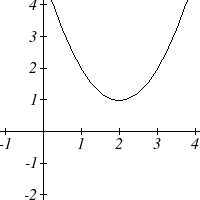
\includegraphics[width=\textwidth]{img/chap1/sec1-5/image058.png}
        \caption{No horizontal intercepts}
    \end{subfigure}
    ~
    \begin{subfigure}[b]{0.3\textwidth}
        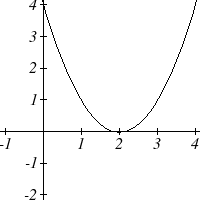
\includegraphics[width=\textwidth]{img/chap1/sec1-5/image059.png}
        \caption{One horizontal intercept}
    \end{subfigure}
    ~
    \begin{subfigure}[b]{0.3\textwidth}
        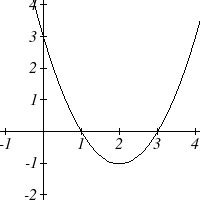
\includegraphics[width=\textwidth]{img/chap1/sec1-5/image060.png}
        \caption{Two horizontal intercepts}
    \end{subfigure}
\end{figure}

Notice that in the standard form of a quadratic, the constant term $c$ reveals the vertical intercept of the graph, since $f(0)=a(0)2+b(0)+c=c$.

\begin{example}
Find the vertical and horizontal intercepts of the quadratic $f(x)=3x^2+5x-2$.

\begin{solution} We can find the vertical intercept by evaluating the function at an input of $0$:
$$f(0)=3(0)^2+5(0)-2=-2 \enspace .$$
So the vertical intercept is at the point $(0,-2)$.

For the horizontal intercepts, we find the 0es (or roots) of $f(x)$, solving $f(x) = 0$ for $x$:
$$0=3x^2+5x-2 \enspace .$$
In this case, the quadratic can be factored easily, providing the simplest method for solution:
$$0=(3x-1)(x+2) \enspace ,$$
so either
\begin{align*}
		0 &= 3x-1\\
		x &= \dfrac{1}{3}
	\end{align*}
or
\begin{align*}
		0 &= x+2\\
		x &= -2
\end{align*}
So the Horizontal intercepts are at the points $\left(\dfrac{1}{3},0\right)$ and $(-2,0)$.
\end{solution}\end{example}

When a quadratic is not factorable or is hard to factor, we can turn to the quadratic formula.

\begin{theorem}[Quadratic Formula]
For a quadratic function given in standard form $f(x)=ax^2+bx+c$, the {\bf quadratic formula}\index{Quadratic formula} gives the horizontal intercepts of the graph of this function:
\[ x=\dfrac{-b\pm \sqrt{b^2-4ac}}{2a} \]
\end{theorem}

\begin{example}
A ball is thrown upwards from the top of a 40 foot high building at a speed of 80 feet per second. The ball's height above ground can be modeled by the equation
$$H(t)=-16t^2+80t+40 \enspace .$$
When does the ball hit the ground?

\begin{solution} To find when the ball hits the ground, we need to determine when the height is 0, i.e., when $H(t)=0$. While we could do this using the transformation form of the quadratic, we can also use the quadratic formula:
\[ t=\dfrac{-80\pm \sqrt{80^2-4(-16)(40)}}{2(-16)}=\dfrac{-80\pm\sqrt{8960}}{-32} \]
Since the square root does not simplify nicely, we can use a calculator to approximate the values of the solutions:
\[ t=\dfrac{-80-\sqrt{8960}}{-32}\approx 5.458 \quad\text{or}\quad t=\dfrac{-80+\sqrt{8960}}{-32}\approx -0.458 \]
The second answer is outside the reasonable domain of our model, so we conclude the ball will hit the ground after about 5.458 seconds.
\end{solution}\end{example}

\subsection{Polynomial Functions}
\label{ssec:polynomial}
% From Section 1.6.

\begin{definition}[Terminology of Polynomial Functions]
A {\bf polynomial}\index{Function!polynomial} is a function that can be written as
\[ f(x)=a_0+a_1 x+a_2 x^2+\ldots +a_n x^n \]
Each of the $a_i$ constants are called {\bf coefficients}\index{Coefficient} and can be positive, negative, or 0, and be whole numbers, decimals, or fractions.

A {\bf term}\index{Term} of the polynomial is any one piece of the sum, that is any $a_ix_i$. Each individual term is a transformed power function.

The {\bf degree}\index{Degree} of the polynomial is the highest power of the variable that occurs in the polynomial.

The {\bf leading term}\index{Term!leading} is the term containing the highest power of the variable: the term with the highest degree.

The {\bf leading coefficient}\index{Coefficient!leading} is the coefficient of the leading term.

Because of the definition of the ``leading" term we often rearrange polynomials so that the powers are descending:
\[ f(x)=a_n x^n+a_{n-1}x^{n-1}\dots a_2 x^2+a_1 x+a_0 \]
\end{definition}
\begin{example}
Identify the degree, leading term, and leading coefficient of the polynomial $f(x)=3+2x^2-4x^3$.

\begin{solution} The degree is 3, the highest power of $x$. The leading term is the term containing that power, $-4x^3$. The leading coefficient is the coefficient of that term, $-4$.
\end{solution}\end{example}

\paragraph*{Short Run Behavior: Intercepts}
As with any function, the {\bf vertical intercept}\index{Intercept!vertical} can be found by evaluating the function at an input of 0. Since this is evaluation, it is relatively easy to do it for a polynomial of any degree. To find {\bf horizontal intercepts}\index{Intercept!horizontal}, we need to solve for when the output will be 0. For general polynomials, this can be a challenging prospect. Consequently, we will limit ourselves to three cases:

\begin{itemize}
	\item The polynomial can be factored using known methods: greatest common factor and trinomial factoring.
	\item The polynomial is given in factored form.
	\item Technology is used to determine the intercepts.
\end{itemize}
\begin{example}
Find the horizontal intercepts of $f(x)=x^6-3x^4+2x^2$.

\begin{solution} We can attempt to factor this polynomial to find solutions for $f(x)=0$:
\begin{align*}
	x^6-3x^4+2x^2    &= 0& &\\
  x^2(x^4-3x^2+2)  &= 0& &\mbox{Factor out the greatest common factor.} \\
  x^2(x^2-1)(x^2-2)&= 0& &\mbox{Factor the inside as a quadratic in } x^2. \\
\end{align*}

Then we break these factors apart to find all the solutions.

\begin{align*}
    x^2 &= 0 & x^2-1 &= 0     & x^2-2 &= 0 \\
		x   &= 0 & x^2   &= 1     & x^2   &= 2 \\
    x   &= 0 & x     &= \pm 1 & x     &= \pm\sqrt{2}
\end{align*}
This gives us five horizontal intercepts: $x=0, \pm 1, \pm \sqrt{2}$.
\end{solution}\end{example}
\begin{example}
Find the horizontal intercepts of $h(t)=t^3+4t^2+t-6$.

\begin{solution} Since this polynomial is not in factored form, has no common factors, and does not appear to be factorable using techniques we know, we can turn to technology to find the intercepts.

Graphing this function, it appears there are horizontal intercepts at $t= -3, -2$, and $1$.

\begin{figure}[!ht]
\centering
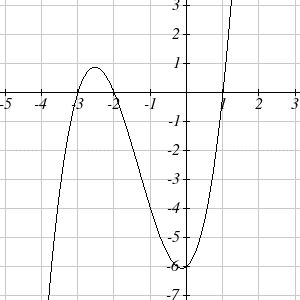
\includegraphics[width=0.4\textwidth]{img/chap1/sec1-5/image067.png}
\caption{}
\end{figure}
We could check these are correct by plugging in these values for $t$ and verifying that $h(-3)=h(-2)=h(1)=0$.
\end{solution}\end{example}
\paragraph*{Solving Polynomial Inequalities}
One application of our ability to find intercepts and sketch a graph of polynomials is the ability to solve polynomial inequalities. It is a very common question to ask when a function will be positive and negative, and one we will use later in this course.

\begin{example}
Solve $(x+3)(x+1)^2(x-4)>0$.

\begin{solution} As with all inequalities, we start by solving the equality $(x+3)(x+1)^2(x-4)=0$, which has solutions at $x= -3, -1$, and $4$. We know the function can only change from positive to negative at these values, so these divide the inputs into four intervals.

We could choose a test value in each interval and evaluate the function $f(x)=(x+3)(x+1)^2(x-4)$ at each test value to determine if the function is positive or negative in that interval:

\begin{table}[!ht]
	\centering
  \begin{tabular}{lrrr}
    \toprule
    Interval     & Test $x$ in interval & $f(x)$ & $ > 0$ or $< 0$?\\
    \midrule
    $x < -3$     & $-4$                 & 72     & $ > 0 $\\
    $-3< x< -1$  & $-2$                 & $-6$   & $ < 0$\\
    $-1 < x < 4$ &   0                  & $-12$  & $ < 0$\\
    $x > 4 $     &   5                  & 288    & $ > 0 $\\
    \bottomrule
\end{tabular}
\end{table}
On a number line this would look like:

\begin{figure}[!ht]
\centering
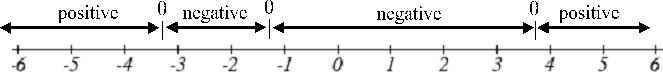
\includegraphics[width=0.4\textwidth]{img/chap1/sec1-5/image068.png}
\caption{}
\end{figure}
From our test values, we can determine this function is positive when $x<-3$ or $x>4$, or in interval notation, $(-\infty,-3)\cup (4,\infty)$.
\end{solution}\end{example}

\subsection{Rational Functions}
\label{ssec:rational}
\begin{definition}
  A {\bf rational function}\index{Function!rational} is the ratio, or fraction, of two polynomials, \(P(x)\) and \(Q(x)\).
	\[f(x)=\dfrac{P(x)}{Q(x)}=\dfrac{a_0+a_1 x+a_2 x^2+\dots+a_p x^p}{b_0+b_1 x+b_2 x^2+\dots+b_q x^q}\].
  \end{definition}
  Rational functions can arise from both simple and complex situations.

\begin{example}
You plan to drive 100 miles. Find a formula for the time the trip will take as a function of the speed you drive.

\begin{solution} You may recall that multiplying speed by time will give you distance. If we let $t$ represent the drive time in hours, and $v$ represent the velocity (speed or rate) at which we drive, then $vt=\mbox{distance}$. Since our distance is fixed at 100 miles, $vt=100$. Solving this relationship for time gives us the function we desired:
$$t(v)=\dfrac{100}{v}\enspace .$$
\end{solution}\end{example}

Notice that this is a transformation of the reciprocal toolkit function, $f(x)=\dfrac{1}{x}$. Several natural phenomena, such as gravitational force and volume of sound, behave in a manner inversely proportional to the square of another quantity. For example, the volume, $V$, of a sound heard at a distance $d$ from the source would be related by $V=\dfrac{k}{d^2}$ for some constant value $k$. These functions are transformations of the reciprocal squared toolkit function $f(x)=\dfrac{1}{x^2}$.

We have seen the graphs of the basic reciprocal function and the squared reciprocal function from our review of toolkit functions. These graphs have several important features.

\begin{figure}[!ht]
\centering
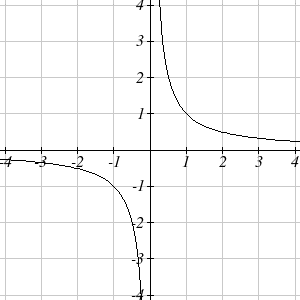
\includegraphics[width=0.4\textwidth]{img/chap1/sec1-5/image070.png}
\caption{$f(x)=\dfrac{1}{x}$}
\end{figure}

\begin{figure}[!ht]
\centering
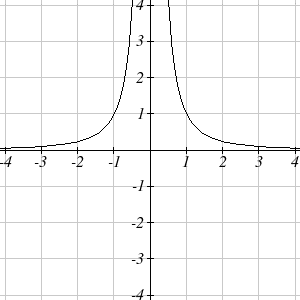
\includegraphics[width=0.4\textwidth]{img/chap1/sec1-5/image069.png}
\caption{$f(x)=\dfrac{1}{x^2}$}
\end{figure}

Let's begin by looking at the reciprocal function, $f(x)=\dfrac{1}{x}$. As you well know, dividing by 0 is not allowed and therefore 0 is not in the domain, and so the function is undefined at an input of 0.

\paragraph*{Short Run Behavior.}
As the input values approach 0 from the left side (taking on very small, negative values), the function values become very large in the negative direction (in other words, they approach negative infinity). We write: $x\to 0^-$, $f(x)\to -\infty$.

As we approach 0 from the right side (small, positive input values), the function values become very large in the positive direction (approaching infinity). We write: as $x\to 0^+$, $f(x)\to\infty$.

This behavior creates a vertical asymptote. An asymptote is a line that the graph approaches. In this case the graph is approaching the vertical line $x=0$ as the input becomes close to 0.

\paragraph*{Long Run Behavior.}
As the values of $x$ approach infinity, the function values approach 0. Also, as the values of $x$ approach negative infinity, the function values approach 0. Symbolically: as $x\to\pm\infty$, $f(x)\to 0$.

Based on this long run behavior and the graph we can see that the function approaches 0 but never actually reaches 0, it just ``levels off" as the inputs become large. This behavior creates a horizontal asymptote. In this case the graph is approaching the horizontal line $f(x)=0$ as the input becomes very large in the negative and positive directions.

\begin{definition}[Vertical and Horizontal Asymptotes]
A {\bf vertical asymptote}\index{Asymptote!vertical} of a graph is a vertical line $x=a$ where the graph tends towards positive or negative infinity as the inputs approach $a$. As $x\to a$, $f(x)\to\pm\infty$.

A {\bf horizontal asymptote}\index{Asymptote!horizontal} of a graph is a horizontal line $y=b$ where the graph approaches the line as the inputs get large. As $x\to\pm\infty$, $f(x)\to b$.
\end{definition}
\begin{example}
Sketch a graph of the reciprocal function shifted two units to the left and up three units. Identify the horizontal and vertical asymptotes of the graph, if any.

\begin{solution} Transforming the graph left 2 and up 3 would result in the function $f(x)=\dfrac{1}{x+2}+3$, or equivalently, by giving the terms a common denominator,
$$f(x)=\dfrac{3x+7}{x+2} \enspace.$$
Shifting the toolkit function would give us this graph. Notice that this equation is undefined at $x=-2$, and the graph also is showing a vertical asymptote at $x=-2$. As $x\to-2^-$, $f(x)\to-\infty$, and as $x\to-2^+$, $f(x)\to\infty$.

\begin{figure}[!ht]
\centering
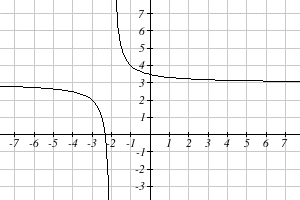
\includegraphics[width=0.4\textwidth]{img/chap1/sec1-5/image071.png}
\caption{}
\end{figure}
As the inputs grow large, the graph appears to be leveling off at output values of 3, indicating a horizontal asymptote at $y=3$. As $x\to\pm\infty$, $f(x)\to 3$
Notice that horizontal and vertical asymptotes get shifted left 2 and up 3 along with the function.
\end{solution}\end{example}

\begin{example}
A large mixing tank currently contains 100 gallons of water, into which 5 pounds of sugar have been mixed. A tap will open pouring 10 gallons per minute of water into the tank at the same time sugar is poured into the tank at a rate of 1 pound per minute. Find the concentration (pounds per gallon) of sugar in the tank after $t$ minutes.

\begin{solution} Notice that the amount of water in the tank is changing linearly, as is the amount of sugar in the tank. We can write an equation independently for each:
$$\text{water}=100+10t \qquad \text{sugar}=5+1t \enspace .$$
The concentration, $C$, will be the ratio of pounds of sugar to gallons of water:
$$C(t)=\dfrac{5+t}{100+10t} \enspace .$$
\end{solution}\end{example}

\paragraph*{Vertical and Horizontal Asymptotes of Rational Functions.}
The {\bf vertical asymptotes} of a rational function will occur where the denominator of the function is equal to 0 and the numerator is not 0.

The {\bf horizontal asymptote} of a rational function, $\dfrac{P(x)}{Q(x)}$ can be determined by looking at the degrees of the numerator, $P(x)$, and the denominator, $Q(x)$.
\begin{itemize}
  \item If $\deg(Q) > \deg(P)$, then the horizontal asymptote is $y=0$.
  \item If $\deg(Q) < \deg(P)$, then there is no horizontal asymptote.
  \item If $\deg(Q) = \deg(P)$, then the horizontal asymptote is $y=\dfrac{a_p}{b_q}$ ($p$ and $q$ are equal in this case).
\end{itemize}

\begin{example}
In the sugar concentration problem from earlier, we created the equation $C(t)=\dfrac{5+t}{100+10t}$. Find the horizontal asymptote and interpret it in context of the scenario.

\begin{solution} Both the numerator and denominator are linear (degree 1), so since the degrees are equal, there will be a horizontal asymptote at the ratio of the leading coefficients. In the numerator, the leading term is $t$, with coefficient 1. In the denominator, the leading term is $10t$, with coefficient 10. The horizontal asymptote will be at the ratio of these values: as $t\to\infty$, $C(t)\to \dfrac{1}{10}$. This function will have a horizontal asymptote of $y=\dfrac{1}{10}$.

This tells us that as the input gets large, the output values will approach $\dfrac{1}{10}$. In context, this means that as more time goes by, the concentration of sugar in the tank will approach 0.1 lb.\ of sugar per gallon of water or $\dfrac{1}{10}$ pounds per gallon.
\end{solution}\end{example}
\begin{example}
Find the horizontal and vertical asymptotes of the function
$$f(x) = \dfrac{(x-2)(x+3)}{(x-1)(x+2)(x-5)} \enspace.$$

\begin{solution} First, note this function has no inputs that make both the numerator and denominator 0, so there are no potential holes. The function will have vertical asymptotes when the denominator is 0, causing the function to be undefined. The denominator will be 0 at $x= 1, -2$, and $5$, indicating vertical asymptotes at these values.

The numerator has degree 2, while the denominator has degree 3. Since the degree of the denominator is greater than the degree of the numerator, the denominator will grow faster than the numerator, causing the outputs to tend towards 0 as the inputs get large, and so as $x\to\pm\infty$, $f(x)\to 0$. This function will have a horizontal asymptote of $y=0$.
\end{solution}\end{example}

As with all functions, a rational function will have a vertical intercept when the input is 0, if the function is defined at 0. It is possible for a rational function to not have a vertical intercept if the function is undefined at 0.

Likewise, a rational function will have horizontal intercepts at the inputs that cause the output to be 0 (unless that input corresponds to a hole). It is possible there are no horizontal intercepts. Since a fraction is only equal to 0 when the numerator is 0, horizontal intercepts will occur when the numerator of the rational function is equal to 0.

\begin{example}
Find the intercepts of
$$f(x)=\dfrac{(x-2)(x+3)}{(x-1)(x+2)(x-5)} \enspace .$$
\begin{solution} We can find the vertical intercept by evaluating the function at 0:
$$f(0)=\dfrac{(0-2)(0+3)}{(0-1)(0+2)(0-5)}=\dfrac{-6}{10}=\dfrac{-3}{5} \enspace .$$
The horizontal intercepts will occur when the function is equal to 0:
\begin{align*}
		0 &= \dfrac{(x-2)(x+3)}{(x-1)(x+2)(x-5)} \qquad \text{(This is zero when the numerator is zero.)}\\
		0 &= (x-2)(x+3)\\
		x &= 2, -3.
\end{align*}
\end{solution}\end{example}
